\documentclass[lettersize,journal]{IEEEtran}
\usepackage{amsmath,amsfonts}
\usepackage{algorithmic}
\usepackage{array}
\usepackage[caption=false,font=normalsize,labelfont=sf,textfont=sf]{subfig}
\usepackage{textcomp}
\usepackage{stfloats}
\usepackage{url}
\usepackage{verbatim}
\usepackage{graphicx}
\usepackage{color}
\hyphenation{op-tical net-works semi-conduc-tor IEEE-Xplore}
\def\BibTeX{{\rm B\kern-.05em{\sc i\kern-.025em b}\kern-.08em
    T\kern-.1667em\lower.7ex\hbox{E}\kern-.125emX}}
\usepackage{balance}

\begin{document}

\title{Distributed Nash Equilibrium Seeking For Second-Order Systems With Boundary Unknown Dynamics}
\author{author
    \thanks{thanks}}

\markboth{Journal of \LaTeX\ Class Files,~Vol.~18, No.~9, September~2020}%
{How to Use the IEEEtran \LaTeX \ Templates}

\maketitle

\begin{abstract}
    This paper investigates the distributed Nash equilibrium seeking problem for second-order systems with unknown dynamics. A chattering free continuous function method is proposed to achieve distributed Nash equilibrium seeking for second-order players by using a time-varying boundary layer technique. The proposed method is able to prevent chattering in practical engineering applications.
    Moreover, by Lyapunov stability analysis, which shows that the proposed method can drive the actions of all players to a small neighborhood of a Nash equilibrium point by adjusting the control gains properly. Finally, a simulation example is provided to verify the result.
\end{abstract}

\begin{IEEEkeywords}
    distributed Nash equilibrium seeking; second-order systems; unknown dynamics; boundary layer technique.
\end{IEEEkeywords}


\section{INTRODUCTION}
\IEEEPARstart{O}{ver}
the past two decades, game theory has spread across diverse research fields, including biology, economics, and computer science. As game theory evolves, the quest for Nash equilibrium in noncooperative games gains significance in theory and practice, as evidenced by studies \cite{pozo2011finding}, \cite{ratliff2016characterization}, \cite{lou2015nash}, \cite{stankovic2011distributed}, \cite{liu2011stochastic}, \cite{durr2013lie}.
Substantial progress has been made in distributed control and optimization of networked systems based on Nash equilibrium seeking and its applications \cite{ding2019distributed}, \cite{wu2021resilient}, \cite{ge2021dynamic}, \cite{ye2022distributed}.
For example, building upon the framework introduced in \cite{7888532}, numerous consensus-based distributed Nash equilibrium seeking strategies have been devised, such as distributed Nash equilibrium seeking in multiagent game under switching communication topologies digraph \cite{8093754} and fully distributed Nash equilibrium seeking \cite{ye2021adaptive}. Nevertheless, the majority of existing findings don't account for the influence of system disturbances, which is unrealistic considering that many practical engineering systems frequently encounter disturbances.

System dynamics are often influenced by external disturbances, leading to significant interest in disturbance attenuation algorithms in engineering applications \cite{7265050}, \cite{xie2000much}, \cite{li2014disturbance}. Common disturbance estimation and attenuation methods include disturbance observer based control, active disturbance rejection control, disturbance accommodation control and composite hierarchical antidisturbance control just a few \cite{7265050}.
For instance, disturbance accommodation control has been widely used in trajectory-driven adaptive control of autonomous unmanned aerial vehicles \cite{prabhakar2018trajectory}, floating offshore wind turbines \cite{namik2009disturbance} and integration of a fuel cell into the power system \cite{paradkar2004integration}.
Furthermore, disturbance attenuation algorithms have been extensively studied in the context of multi-agent systems.
For instance, an event-triggered control strategy to solve the security consensus problem for multi-agent systems under multiple disturbances and false data injection attacks \cite{9745491}. A distributed observer was designed for each agent to estimate the desired tracking signal that address the distributed average tracking problem for linear multi-agent systems with heterogeneous dynamics and external disturbances \cite{9547799}. There are two containment control protocols, one is based on a terminal sliding mode and  the other is based on a non-singular terminal sliding mode, has been developed to finite-time containment control for nonlinear multi-agent systems with external disturbances \cite{LU2020338}. With the aid of sliding-mode control technique, distributed finite-time tracking control for nonlinear multi-agent systems subject to external disturbances can achieve  the finite convergence time is explicitly presented \cite{zhang2013distributed}.

Inspired by the significance of disturbance attenuation algorithms in practical engineering applications, distributed Nash equilibrium seeking strategies were proposed based on reduced-order disturbance observers and signum function \cite{9696299}, extended state observer \cite{ye2020distributed}, unknown dynamics estimator \cite{li2021distributed}.
This paper aims to address the distributed Nash equilibrium seeking problem for second-order systems with unknown boundary disturbances by a chattering free continuous function method. Compared to most of existing literature, this paper's contributions are summarized as follows:
\begin{enumerate}
    \item This paper proposes a chattering free continuous function method by using a time-varying boundary layer technique that achieve disturbance rejection distributed Nash equilibrium seeking for second-order players. The proposed method is able to prevent chattering in practical engineering applications, which is in contrast to the signum function method in \cite{9696299}.Moreover, the method in \cite{8985536} requires distributed estimation of all players' actions and some specific objective functions determined by the players, while the proposed method in this paper does not. Therefore, compared to the methods in \cite{9696299}, \cite{ye2020distributed}, \cite{li2021distributed}, \cite{8985536}, the proposed method in this paper requires less computation.
    \item Due to high frequency switching of discontinuous terms, the controller may induce chattering in practical implementations which is detrimental to actuators. Compared \cite{9696299}, this paper proposes a continuous function method, chattering is avoided.
    \item By Lyapunov stability analysis, which shows that the proposed method can drive the actions of all players to a small neighborhood of a Nash equilibrium point by adjusting the control gains properly.
\end{enumerate}

The rest of this paper is organized as follows. Section II gives notations and preliminaries. Problem statement is introduced in Section III and main results are given in Section IV where we utilize boundary layer technique to design a continuous function method for distributed Nash equilibrium seeking for second-order players. Simulation studies are presented in Section V and conclusions are drawn in Section VI.


\section{NOTATIONS AND PRELIMINARIES}
\emph{Notations}: The real number set is denote as $\mathbb{R}$. $\|z\|$ denotes the $\ell_2-$norm of z. $[z_i]_{vec}$ where $i \in \{1,2,...,N\}$ is defined as a column vector whose dimension is $N \times 1$ and the $i$th element is $z_i$. diag$\{k_i\}$ for $i \in \{1,2,...,N\}$ is a diagonal matrix whose dimension is $N\times N$ and the $i$th diagonal element is $k_i$. diag$\{a_{ij}\}$ where $i,j \in \{1,2,...,N\}$ gives a diagonal matrix whose dimension is $N^2 \times N^2$ and diagonal elements are $a_{11},a_{12},...,a_{1N},a_{21},...,a_{NN}$, successively. $\mathcal{A} = [a_{ij}]$ is a matrix whose $(i,j)$th entry is $a_{ij}$. Given that matrix $Q$ is symmetric and real, $\lambda_{min}(Q)(\lambda_{max}(Q))$ stands for the smallest(largest) eigenvalue of $Q$. $max_{i \in \{1,2,...,N\}}\{l_i\}$ denotes the largest value of $l_i$ for $i \in \{1,2,...,N\}$. $\mathbf{I}_{N \times N}$ is an identity matrix with its dimension being $N \times N$ and $\mathbf{1}(\mathbf{0})$ is a column vector with its entries being 1(0). Moreover, $\otimes$ is the Kronecker product.

\emph{Algebraic Graph Theory}: A graph $\mathcal{G}$ is given by $\mathcal{G} = (\mathcal{V},\mathcal{E}_g)$, in which $\mathcal{V} = \{1,2,...,N\}$, $\mathcal{E}_g \subseteq \mathcal{V}\times\mathcal{V}$ respectively are the node set and edge set. The edge $(i,j) \in \mathcal{E}_g$ indicates are the node $j$ can receive information from node $i$, but not necessarily vice versa. The in-neighbor set of node $i$ is given as $\mathcal{N}_{i}^{in}=\{j|(j,i)\in\mathcal{E}_{g}\}$. A directed path is a sequence of edges of the form $(i_1,i_2), (i_2,i_3),....$ A directed graph is strongly connected if for every pair of two distinct nodes, there is a path. Let $\mathcal{A} = [a_{ij}]$ be the adjacency matrix in which $a_{ij} > 0$ if $(i,j) \in \mathcal{E}_g$ and $a_{ij} = 0$ otherwise. The Laplacian matrix $\mathcal{L}$ is defined as $\mathcal{L} = \mathcal{D} - \mathcal{A}$ \cite{lewis2013cooperative}, where $\mathcal{D} = \text{diag}\{d_i\}$ and $d_i = \sum_{j=1}^{N}a_{ij}$.


\section{PROBLEM STATEMENT}
In the concerned game, $N$ players with labels from $1$ to $N$ are engaged and each player $i$ has a local objective function $f_i(\mathbf{x}):\mathbb{R}^N \rightarrow \mathbb{R}$, in which $\mathbf{x} = [x_1,x_2,...,x_N]^T$ and $x_i \in \mathbb{R}$ is the action of player $i$\footnote{
    For the sake of simplicity in presentation, let's assume that $x_i$ is one-dimensional. However, it is important to note that the methods and results presented herein are directly applicable to accommodate games with multi-dimensional actions.
}.
Moreover, for second-order players, player $i$'s action is governed by
\begin{equation}\label{eq1}
    \begin{cases}
        \dot{x}_i(t)=v_i(t) \\
        \dot{v}_i(t)=u_i+d_i(t)
    \end{cases}
\end{equation}
where $v_i(t)$ is the velocity-like state of player $i$, $u_i$ is the control input and $d_i(t)$ is the disturbance for $i \in \mathcal{V}$. Each player $i$ aims to minimize its own objective function $f_i(\mathbf{x})$ by adjusting its action $x_i(t)$, that is
\begin{equation}
    \begin{aligned}
        \min_{x_i}  ~ & f_i(\mathbf{x})        \\
        \text{s.t.} ~ & \begin{cases}
                            \dot{x}_i(t)=v_i(t) \\
                            \dot{v}_i(t)=u_i+d_i(t)
                        \end{cases}
    \end{aligned}
\end{equation}

\emph{Definition 1}: Nash equilibrium is an action profile on which no player can gain more payoff by unilaterally changing its own action, i.e., an action profile $\mathbf{x}^{*}=(x_{i}^{*},\mathbf{x}_{-i}^{*})$ is a Nash equilibrium if for all $i \in \mathcal{V}$, we have
\begin{equation}
    f_i(x_i^*,\mathbf{x}_{-i}^*)\leq f_i(x_i,\mathbf{x}_{-i}^*),\forall x_i\in\mathbb{R}
\end{equation}
where $\mathbf{x}_{-i}=[x_{1},x_{2},\ldots,x_{i-1},x_{i+1},\ldots,x_{N}]^{T}$.

To streamline the forthcoming analysis, the following assumptions are employed.

\emph{Assumptions 1}: For $i \in \mathcal{V}$, $f_i(\mathbf{x})$ is $\mathcal{C}^2$ and $\nabla f_i(\mathbf{x})$ is globally Lipschitz with $l_i$.

\emph{Assumptions 2}: The digraph $\mathcal{G}$ is strongly connected among the players.

\emph{Lemma 1} \cite{lewis2013cooperative}: Let $D$ be a nonnegative diagonal matrix and $\mathcal{H} = \mathcal{L} + D$. Under Assumptions 2, there are symmetric positive definite matrices $P$ and $Q$ such that
\begin{equation}
    \mathcal{H}^{T}P+P\mathcal{H}=Q
\end{equation}

\emph{Assumptions 3}: For $\mathbf{x}, \mathbf{z} \in \mathbb{R}^N$,
\begin{equation}
    (\mathbf{x}-\mathbf{z})^T([\nabla_if_i(\mathbf{x})]_{vec}-[\nabla_if_i(\mathbf{z})]_{vec})\geq m\|\mathbf{x}-\mathbf{z}\|^2
\end{equation}
where $\nabla_{i}f_{i}(\mathbf{x})=\partial f_{i}(\mathbf{x})/\partial x_{i}$ and $m$ is a positive constant.

\emph{Remark 1}: Assumption 1 ensures that the players' objective functions are sufficiently smooth. Moreover, the global Lipschitzness $\nabla_if_i(\mathbf{x})$ is employed to develop global results and it can be removed with the corresponding results degraded to be semi-global ones. Assumption 2 is utilized to ensure players can broadcast their local information to the other players through neighboring communication, which enables the distributed estimation of the players' actions. The strong monotonicity condition in Assumption 3 ensures the existence of a unique Nash equilibrium, on which $[\nabla_if_i(\mathbf{x}^*)]_{vec} = \mathbf{0}_N$ \cite{ye2020distributed}.
It's worth mentioning that Assumption 1-3 are widely adopted in the exist literature \cite{8093754}, \cite{ye2021adaptive}, \cite{9696299}, \cite{ye2020distributed}, \cite{li2021distributed}, \cite{8985536}.
Moreover, together with Assumption 1, Assumption 3 ensures that the Nash equilibrium is globally exponentially stable under the gradient play given by
\begin{equation}
    \dot{x}_i=-\nabla_if_i(\mathbf{x}),~ i \in \mathcal{V}
\end{equation}
which is the core idea behind the design of the seeking strategies \cite{7888532}.

\section{MAIN RESULTS}
In this section, a chattering free continuous function method is proposed to achieve distributed Nash equilibrium seeking for second-order players by using a time-varying boundary layer technique.

Motivated by \cite{7888532}, \cite{9696299}, \cite{10192924}, to realize asymptotic Nash equilibrium seeking for games with second-order integrator-type players distributively, the control input is designed as
\begin{equation}\label{eq7}
    \begin{cases}
        u_i=-\tau k_ih_i-\beta_i\xi_i(t)                                                                      \\
        h_i=v_i+\nabla_if_i(\mathbf{y}_i)                                                                     \\
        \dot{y}_{ij}=-\theta\bar{\theta}_{ij}\Bigg(\sum_{k=1}^Na_{ik}(y_{ij}-y_{kj})+a_{ij}(y_{ij}-x_j)\Bigg) \\
        \dot{\varrho}_i(t) = -\alpha_i \varrho_i(t)~\text{with}~\varrho_i(t) > 0
    \end{cases}
\end{equation}
where $i,j \in \mathcal{V},~ \theta, ~\tau$ are adjustable positive parameters, $\bar{\theta}_{ij},~ k_i,~ \alpha_i$ are fixed positive parameters, $\beta_i \geq \bar{d}_i$ is a positive constant, $y_{ij}$ represents player $i$'s estimate on $x_j$, $\mathbf{y}_i = [y_{i1}, y_{i2},..., y_{iN}]^T$, $h_i$ and $\varrho_i(t)$ represents an auxiliary variable for player $i$ and let $\xi_i(t) = h_i(t)/(|h_i(t)| + \varrho_i(t))$.

\emph{Remark 2}: The control law (\ref{eq7}) is distributed, with each player only relying on its own information (e.g., gradient and action data) and information from its neighboring nodes in the communication network to update its own action. Furthermore the control input consists of two parts: $-\beta_i\xi_i(t)$ is used to compensate for the disturbances, and $-\nabla_if_i(\mathbf{y}_i)$ is a gradient-like term that is used to drive the players' actions to optimize their own objective functions.

By (\ref{eq1}) and (\ref{eq7}), the closed-loop system is
\begin{equation}\label{eq8}
    \begin{cases}
        \dot{\mathbf{x}}=\mathbf{v}                                                      \\
        \dot{\mathbf{v}}=-\tau\mathbf{k}\mathbf{h}-[\beta_i\xi_i(t)]_{vec}+\mathbf{d}(t) \\
        \mathbf{h}=\mathbf{v}+[\nabla_if_i(\mathbf{y}_i)]_{vec}                          \\
        \dot{\mathbf{y}}=-\theta\bar{\theta}(\mathcal{L}\otimes\mathbf{I}_{N\times N}+\mathcal{A}_q)\tilde{\mathbf{y}}
    \end{cases}
\end{equation}
where $\mathbf{k} = \text{diag}\{k_i\},~
    \bar{\mathbf{\theta}} = \text{diag}\{\bar{\theta}_{ij}\},~
    \mathcal{A}_q = \text{diag}\{a_{ij}\}, ~\mathbf{y} = [\mathbf{y}_1^T,\mathbf{y}_2^T,...,\mathbf{y}_N^T]^T$ and $\tilde{\mathbf{y}} = \mathbf{y} - \mathbf{1}_N \otimes \mathbf{x}$. From Assumption 2 and Lemma 1, it can be obviously deduced that they are positive diagonal matrices $P,Q\in\mathbb{R}^{N^{2}\times N^{2}}$ in order to $Q = P\bar{\theta}(\mathcal{L}\otimes\mathbf{I}_{N\times N}+\mathcal{A}_q)+(\mathcal{L}\otimes\mathbf{I}_{N\times N}+\mathcal{A}_q)^T\bar{\theta}P$.

To proceed with the forthcoming analysis, we make the following assumption.

\emph{Assumptions 4}: For $i \in \mathcal{V}$, $\nabla_{ij}^{2}f_{i}(\mathbf{x})=\partial^{2}f_{i}(\mathbf{x})/\partial x_{i}\partial x_{j}$ is bounded.

To establish the convergence result, we assume that the disturbances possess the following property.

\emph{Assumptions 5}: The disturbance $d(t)$ is bounded, i.e., $\forall i \in \mathcal{V}, |d_i(t)|\leq \bar{d}_i(t)$ for a positive constant $\bar{d}_i$.

Let $\tilde{\mathbf{x}} = \mathbf{x} - \mathbf{x}^*$. Then, the subsequent result can be derived.

\emph{Theorem 1}: Under Assumptions 1-5, there exist a $\theta^* > 0$ such that for each $\theta > \theta^*$, there exists a $\tau^* > 0$ such that for each $\tau > \tau^*$, players' actions globally exponentially converge to the Nash equilibrium by (\ref{eq8}).

\begin{IEEEproof}
    Define $V = V_1 + V_2 + V_3$, where
    \begin{equation}
        \begin{aligned}
            V_1(t) & = \frac{1}{2}\tilde{\mathbf{x}}^{T}\tilde{\mathbf{x}}                                         \\
            V_2(t) & = \frac{1}{2}\tilde{\mathbf{y}}^{T}P\tilde{\mathbf{y}}                                        \\
            V_3(t) & = \frac{1}{2}\mathbf{h}^{T}\mathbf{h} + \sum_{i = 1}^{N} \frac{\beta_i}{\alpha_i}\varrho_i(t)
        \end{aligned}
    \end{equation}

    Then, taking the time derivative of $V_1$ yields
    \begin{equation}
        \begin{aligned}
            \dot{V}_{1} & =\tilde{\mathbf{x}}^{T}(\mathbf{h}-[\nabla_{i}f_{i}(\mathbf{y}_{i})]_{vec})                                                                   \\
                        & \leq-m\|\tilde{\mathbf{x}}\|^2+\max_{i\in\mathcal{V}}\{l_i\}\|\tilde{\mathbf{x}}\|\|\tilde{\mathbf{y}}\|+\|\tilde{\mathbf{x}}\|\|\mathbf{h}\|
        \end{aligned}
    \end{equation}
    where in the inequality, we have used Assumptions 3 and $\|[\nabla_{i}f_{i}(\mathbf{y}_{i})]_{vec}-[\nabla_{i}f_{i}(\mathbf{x})]_{vec}\|\leq\max_{i\in\mathcal{V}}\{l_{i}\}\|\tilde{\mathbf{y}}\|$.

    Then, taking the time derivative of $V_2$ yields
    \begin{equation}
        \begin{aligned}
            \dot{V}_{2}= & \dot{\tilde{\mathbf{y}}}^{T}P\tilde{\mathbf{y}}+\tilde{\mathbf{y}}^{T}P\dot{\tilde{\mathbf{y}}}                                         \\
            =            & -\theta\tilde{\mathbf{y}}^TQ\tilde{\mathbf{y}}-2\tilde{\mathbf{y}}^TP\mathbf{1}_N\otimes\mathbf{h}                                      \\
                         & +2\tilde{\mathbf{y}}^TP\mathbf{1}_N\otimes[\nabla_if_i(\mathbf{y}_i)]_{vec}                                                             \\
            \leq         & -(\theta\lambda_{\min}(Q)-2\sqrt{N}\|P\|\max_{i\in\mathcal{V}}\{l_{i}\})\|\tilde{\mathbf{y}}\|^{2}                                      \\
                         & +2\sqrt{N}\|P\|\|\tilde{\mathbf{y}}\|\|\mathbf{h}\|+2N\|P\|\max_{i\in\mathcal{V}}\{l_{i}\}\|\tilde{\mathbf{y}}\|\|\tilde{\mathbf{x}}\|.
        \end{aligned}
    \end{equation}
    where in the inequality, by Assumption 2 and Lemma 1, we let $P,Q\in\mathbb{R}^{N^{2}\times N^{2}}$ and $Q = P\bar{\theta}(\mathcal{L}\otimes\mathbf{I}_{N\times N}+\mathcal{A}_q)+(\mathcal{L}\otimes\mathbf{I}_{N\times N}+\mathcal{A}_q)^T\bar{\theta}P$.

    Moreover, taking the time derivative of $V_3$ yields
    \begin{equation}
        \begin{aligned}
            \dot{V}_3  = & {\mathbf{h}}^T(\dot{\mathbf{v}}+\bar{H}(\mathbf{y})\dot{\mathbf{y}}) - \sum_{i = 1}^{N} \beta_i\varrho_i(t)          \\
            =            & {\mathbf{h}}^T(-\tau\mathbf{k}\mathbf{h}-[\beta_i\xi_i(t)]_{vec}+\mathbf{d}(t) +\bar{H}(\mathbf{y})\dot{\mathbf{y}}) \\
                         & - \sum_{i = 1}^{N} \beta_i\varrho_i(t)
        \end{aligned}
    \end{equation}
    where $\bar{H}(\mathbf{y})=[h_{ij}]$ in which for $i \neq j$, $h_{ij} = \mathbf{0}_N^T$ and for $i = j$, $h_{ii}=[\nabla_{i1}^{2}f_{i}(\mathbf{y}_{i}),\nabla_{i2}^{2}f_{i}(\mathbf{y}_{i}),\ldots,\nabla_{iN}^{2}f_{i}(\mathbf{y}_{i})]$, $\nabla_{ij}^{2}f_{i}(\mathbf{y}_{i})=\frac{\partial^{2}f_{i}(\mathbf{x})}{\partial x_{i}\partial x_{j}}\mid_{\mathbf{x}=\mathbf{y}_{i}}$. By Assumption 4, $\|\bar{H}\mathbf{y}\|$ is bounded. Hence, There are some positive constant $L_1$ meet $\|\bar{H}(\mathbf{y})\|\|\bar{\boldsymbol{\theta}}(\mathcal{L}\otimes \mathbf{I}_{N\times N}+\mathcal{A}_{q})\|\leq L_{1}$. Therefore,
    \begin{equation}
        \begin{aligned}
            \dot{V}_3 & \leq-\tau\lambda_{\min}(\mathbf{k})\|{\mathbf{h}}\|^2+\theta L_1\|{\mathbf{h}}\|\|\tilde{\mathbf{y}}\|                       \\
                      & -\sum_{i = 1}^{N}\frac{(\beta_i - |d_i(t)|)|h_i(t)|(|h_i(t)|+\varrho_i(t)) + \beta_i\varrho_i^2(t)}{|h_i(t)| + \varrho_i(t)}
        \end{aligned}
    \end{equation}

    Hence,
    \begin{equation}
        \begin{aligned}
            \dot{V}\leq & -m\|\tilde{\mathbf{x}}\|^2-\tau\lambda_{\min}(\mathbf{k})\|\mathbf{h}\|^2                                                    \\
                        & -(\theta\lambda_{\min}(Q)-2\sqrt{N}\|P\|\max_{i\in\mathcal{V}}\{l_i\})\|\tilde{\mathbf{y}}\|^2                               \\
                        & +(\max_{i\in\mathcal{V}}\{l_i\}+2N\|P\|\max_{i\in\mathcal{V}}\{l_i\})\|\tilde{\mathbf{x}}\|\|\tilde{\mathbf{y}}\|            \\
                        & +(2\sqrt{N}\|P\|+\theta L_{1})\|\tilde{\mathbf{y}}\|\|\mathbf{h}\|+\|\tilde{\mathbf{x}}\|\|\mathbf{h}\|                      \\
                        & -\sum_{i = 1}^{N}\frac{(\beta_i - |d_i(t)|)|h_i(t)|(|h_i(t)|+\varrho_i(t)) + \beta_i\varrho_i^2(t)}{|h_i(t)| + \varrho_i(t)} \\
            \leq        & -\lambda_{\min}(F)\|\mathbf{E}_1\|^2-\tau\lambda_{\min}(\mathbf{k})\|\mathbf{h}\|^2                                          \\
                        & +(1+2\sqrt{N}\|P\|+\theta L_1)\|\mathbf{E}_1\|\|\mathbf{h}\|
        \end{aligned}
    \end{equation}
    where $\left.F=\left[\begin{array}{cc}m & a                                                                   \\
             a     & \theta\lambda_{\min}(Q)-2\sqrt{N}\|P\|\max_{i\in\mathcal{V}}\{l_i\}\end{array}\right.\right]$,
    $\mathbf{E}_1 = [\tilde{\mathbf{x}}^T,\tilde{\mathbf{y}}^T]^T$,
    ~~~$a = -\frac{\max_{i\in\mathcal{V}}\{l_{i}\}+2N\|P\|\max_{i\in\mathcal{V}}\{l_{i}\}}{2}$, choose
    $\theta > \frac{(\max_{i\in\mathcal{V}}\{l_{i}\}+2N\|P\|\max_{i\in\mathcal{V}}(l_{i}\})^{2}}{4m\lambda_{\mathrm{min}}(Q)}+\frac{2\sqrt{N}\|P\|\max_{i\in\mathcal{V}}\{l_{i}\}}{\lambda_{\mathrm{min}}(Q)}$. Then, $\lambda_{min}(F)$ is a real positive number and $\lambda_{min}(F) > 0$. Thus,
    \begin{equation}
        \dot{V}(t) \leq -\lambda_{\min}(G)\|\mathbf{E}\|^2
    \end{equation}
    where $\left.G=\left[\begin{array}{cc}\lambda_{\min}(F)&-\frac{1+2\sqrt{N}\|P\|+\theta L_1}2\\-\frac{1+2\sqrt{N}\|P\|+\theta L_1}2&\tau\lambda_{\min}(\mathbf{k})\end{array}\right.\right],
        \mathbf{E} = [\tilde{\mathbf{x}}^T,\tilde{\mathbf{y}}^T,\tilde{\mathbf{h}}^T]^T$. By choosing
    $\tau>\frac{(1+2\sqrt{N}\|P\|+\theta L_{1})^{2}}{4\lambda_{\mathrm{min}}(F)\lambda_{\mathrm{min}}(\mathbf{k})}$, $\lambda_{min}(G)$ is a real positive number and $\lambda_{min}(G) > 0$.

    According to the definition of Lyapunov candidate function, the conclusion can be drawn.
\end{IEEEproof}

\emph{Remark 3}: Theorem 1 indicates that for any initial condition, the presented algorithm can drive the actions of all players to a small neighborhood of a Nash equilibrium point by adjusting the control gains $\tau$ and $\theta$ properly.



\section{SIMULATION STUDIES}
This section provides a simulation example to verify the effectiveness of the proposed method. Consider a game with $5$ players, where the objective functions are given by
\begin{equation*}
    \begin{aligned}
        f_1(\mathbf{x}) = & \|x_1-\mathbf{1}_2\|^2+(x_{11}+x_{21})^2+(x_{12}-x_{22})^2                                \\
                          & +\left\|x_1+x_3\right\|^2+\left(x_{11}-x_{41}\right)^2+\left(x_{12}+x_{42}\right)^2       \\
                          & +\|x_1-\mathbf{1}_2-x_5\|^2                                                               \\
        f_2(\mathbf{x}) = & (x_{21}+1)^2+(x_{22}-1)^2+(x_{21}+x_{11})^2                                               \\
                          & +(x_{22}-x_{12})^2+(x_{21}-x_{31})^2+(x_{22}+x_{32})^2                                    \\
                          & +\|x_2+x_4\|^2+(x_{21}+1-x_{51})^2+(x_{22}-1-x_{52})^2                                    \\
        f_3(\mathbf{x}) = & \|x_3+\mathbf{1}_2\|^2+\|x_3+x_1\|^2+(x_{31}-x_{21})^2                                    \\
                          & +(x_{32}+x_{22})^2+(x_{31}+x_{41})^2                                                      \\
                          & +(x_{32}-x_{42})^2+\|x_3+\mathbf{1}_2-x_5\|^2                                             \\
        f_4(\mathbf{x}) = & (x_{41}-1)^2+(x_{42}+1)^2+(x_{41}-1-x_{51})^2                                             \\
                          & +\|x_4+x_2\|^2+(x_{41}+x_{31})^2+(x_{42}-x_{32})^2                                        \\
                          & +\left(x_{42}+1-x_{52}\right)^2+\left(x_{41}-x_{11}\right)^2+\left(x_{42}+x_{12}\right)^2 \\
        f_5(\mathbf{x}) = & \|x_5\|^2+\|x_5+\mathbf{1}_2-x_1\|^2+(x_{51}+1+x_{21})^2                                  \\
                          & +(x_{52}+1-x_{22})^2+\|x_5+\mathbf{1}_2+x_3\|^2                                           \\
                          & +(x_{51}+1-x_{41})^2+(x_{52}+1+x_{42})^2
    \end{aligned}
\end{equation*}
where $x_i = [x_{i1}, x_{i2}]^T$, and $\mathbf{x}=[x_1^T,x_2^T,x_3^T,x_4^T,x_5^T]^T$. In addition, we study a network consisting of $5$ players whose communication topology is shown in Fig. 1.
\begin{figure}[htbp]
    \centering
    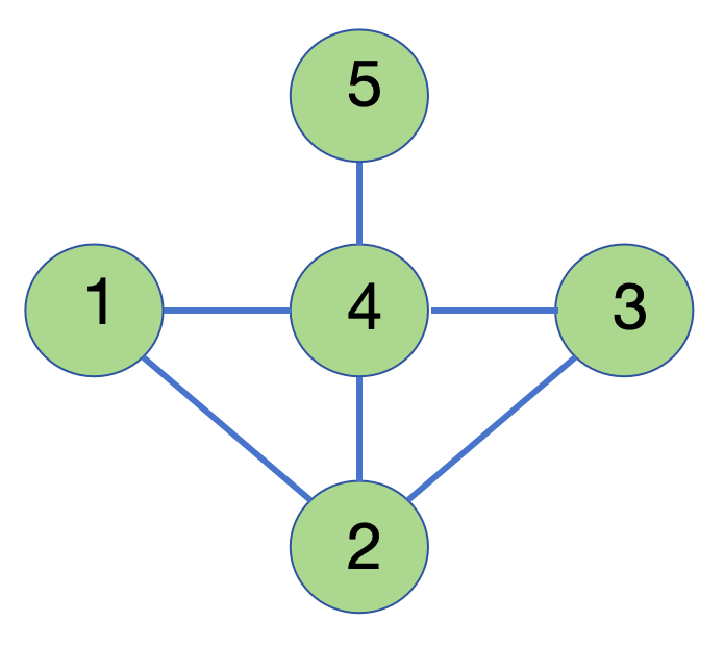
\includegraphics[width=0.3\textwidth]{img/fig1.eps}
    \caption{Communication topology of the network.}
\end{figure}

By calculation, it is found that $\mathbf{x}^* = [0.8,0.2,-0.7,0.4,\\
    -0.7,-0.55,0.8,-0.7,-0.2,-0.4]^T$,
and the proposed algorithm (\ref{eq7}) will be verified with $\mathbf{x}(0) = [2.5,-2.5,0,2,4,5,\\0.5,-4,-3.5,-2.5]^T$. Moreover, all the other variables are initialized at zero and the disturbance vector is considered to be $\mathbf{d}(t)=[2\sin(t),2\sin(t),2\cos(t),2\cos(t),4\cos(2t),\\4\cos(2t),4\sin(2t),4\sin(2t),6\sin(3t),6\sin(3t)]^T$.

The algorithm (\ref{eq7}) is simulated with $\tau k_i = 9,~\theta\overline{\theta}_{ij}=70,~\alpha_i = 1,~i\in \{1,2,3,4,5\},~j\in \{1,2\}$. The results are shown in Fig. 2, Fig. 3 and Fig. 4, they represents players' actions $x_{i1}, ~x_{i2}$ and players' velocity-like state $v_{ij}$ for $i\in \{1,2,3,4,5\},~j\in \{1,2\}$.
\begin{figure}[htbp]
    \centering
    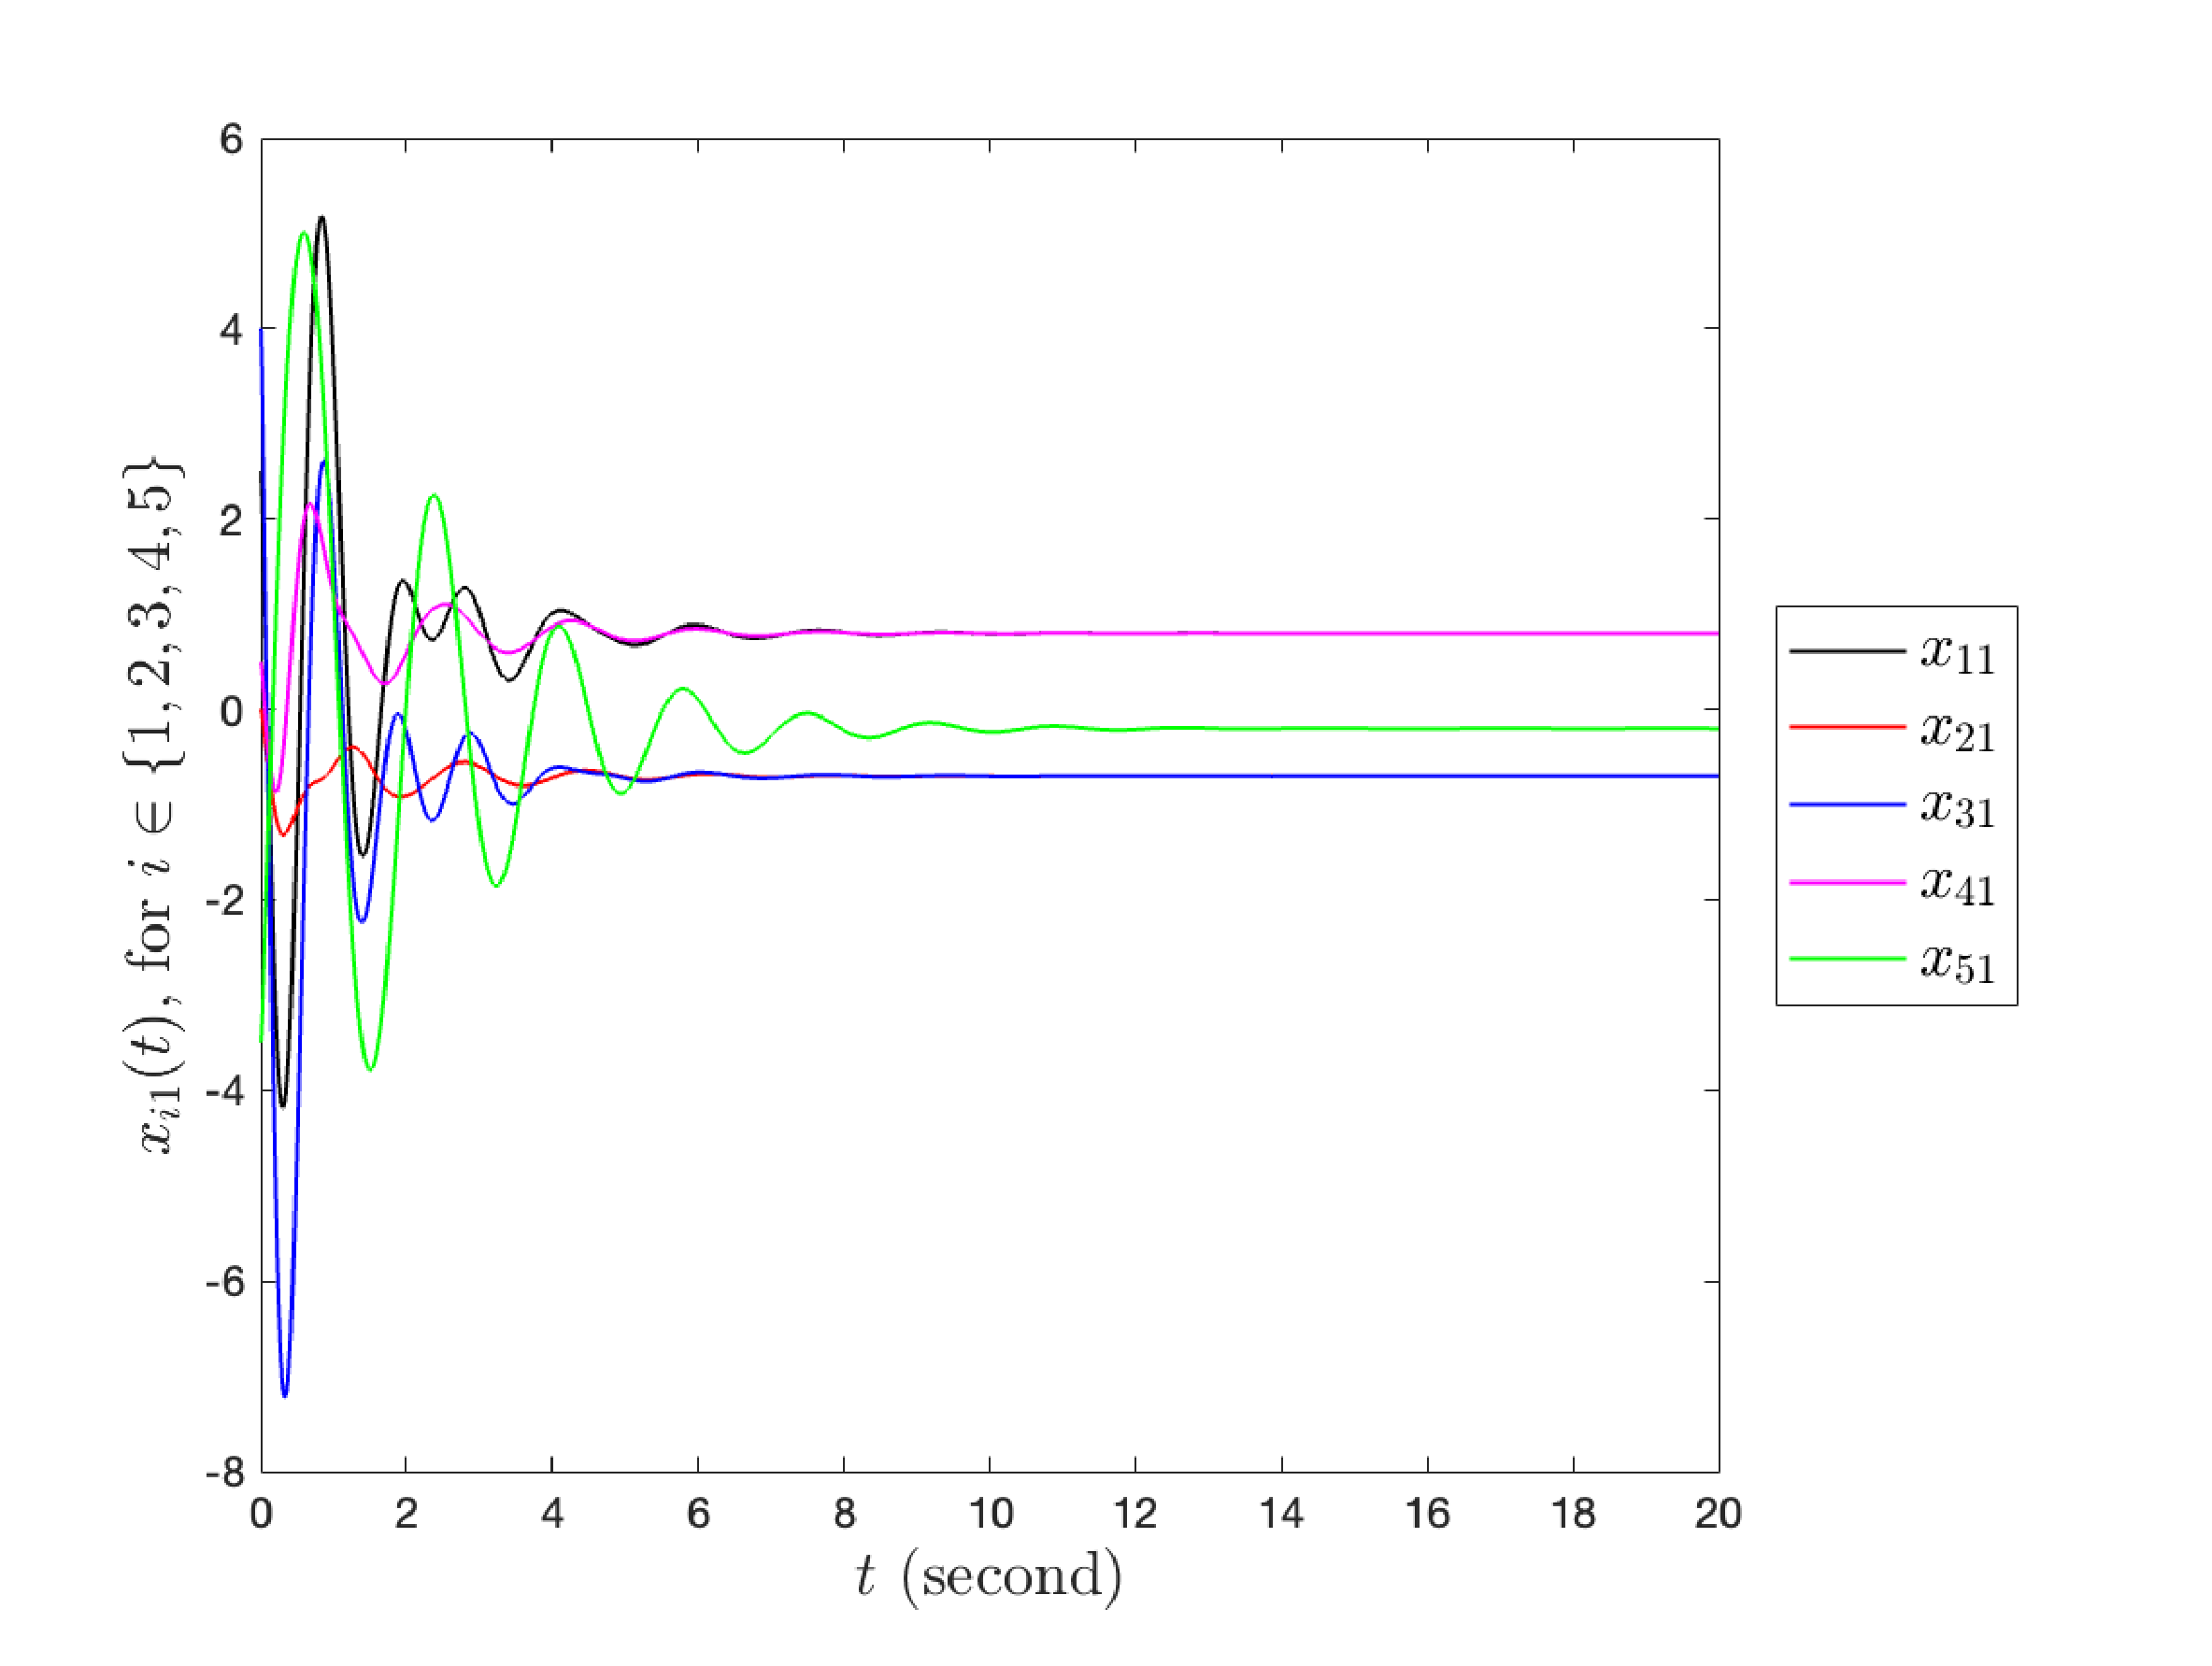
\includegraphics[width=0.45\textwidth]{img/xi1.eps}
    \caption{Players' actions $x_{i1}$ for $i\in \{1,2,3,4,5\}$.}
\end{figure}

\begin{figure}[htbp]
    \centering
    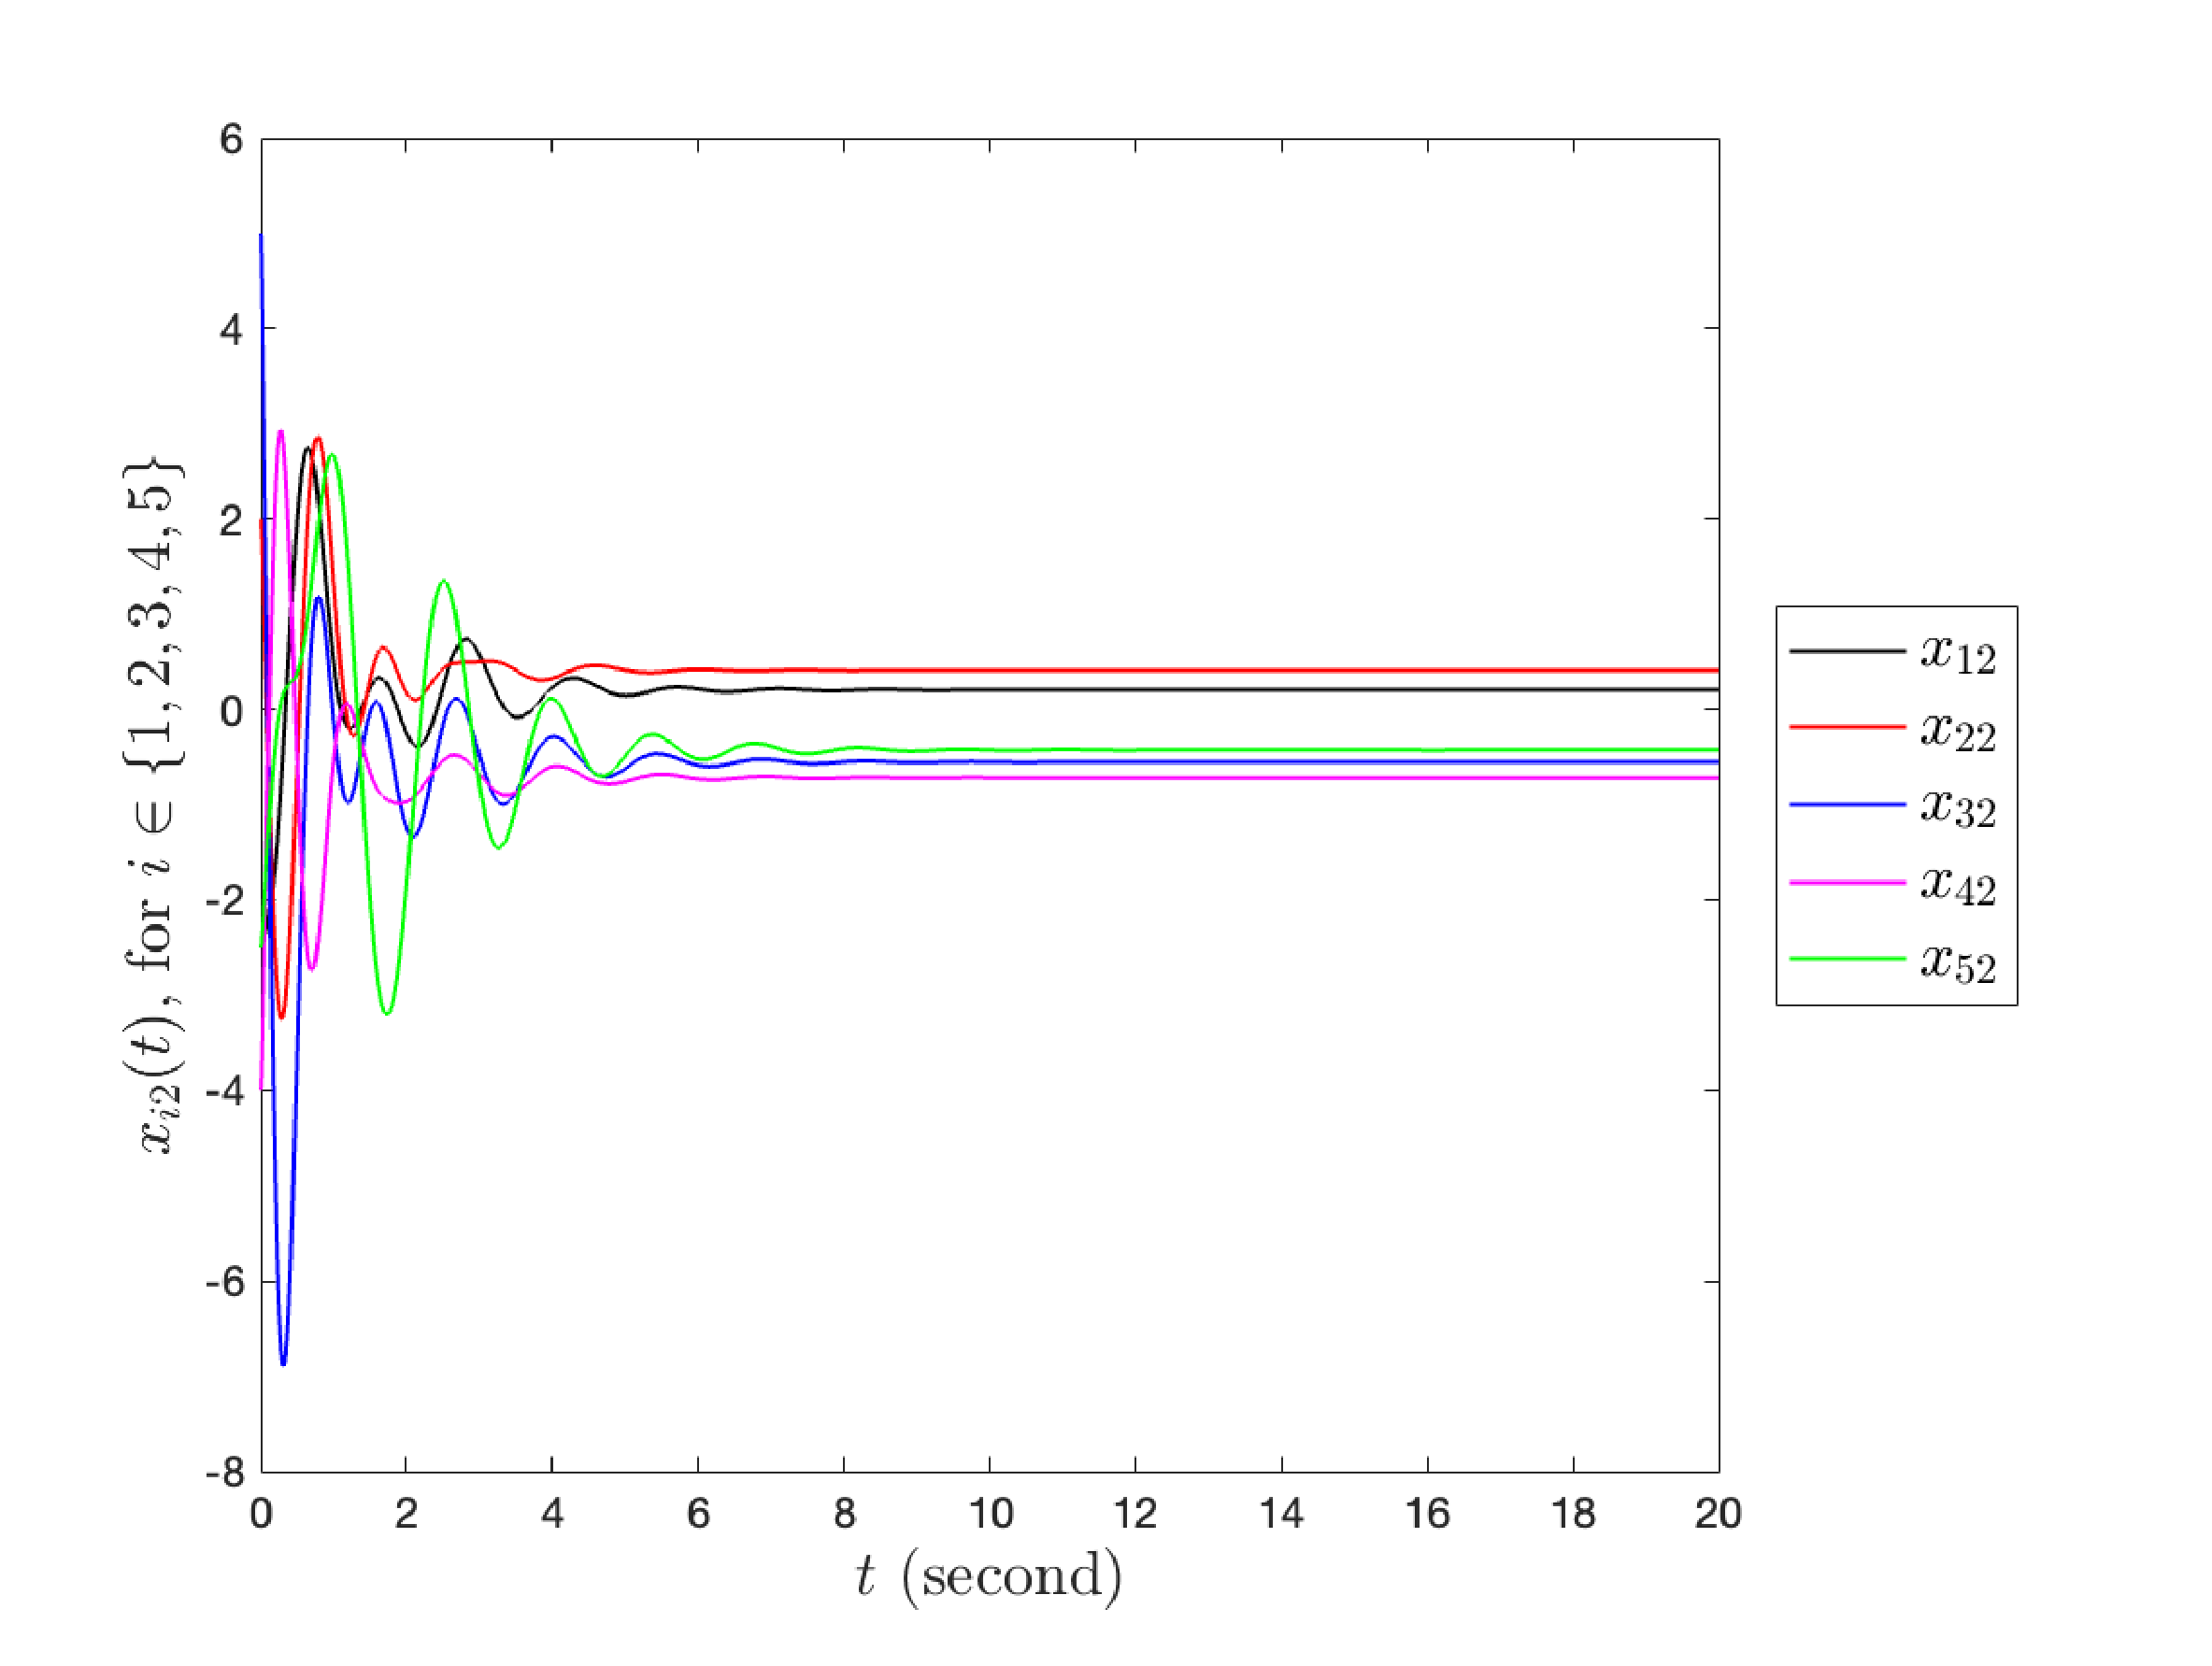
\includegraphics[width=0.45\textwidth]{img/xi2.eps}
    \caption{Players' actions $x_{i2}$ for $i\in \{1,2,3,4,5\}$.}
\end{figure}

\begin{figure}[htbp]
    \centering
    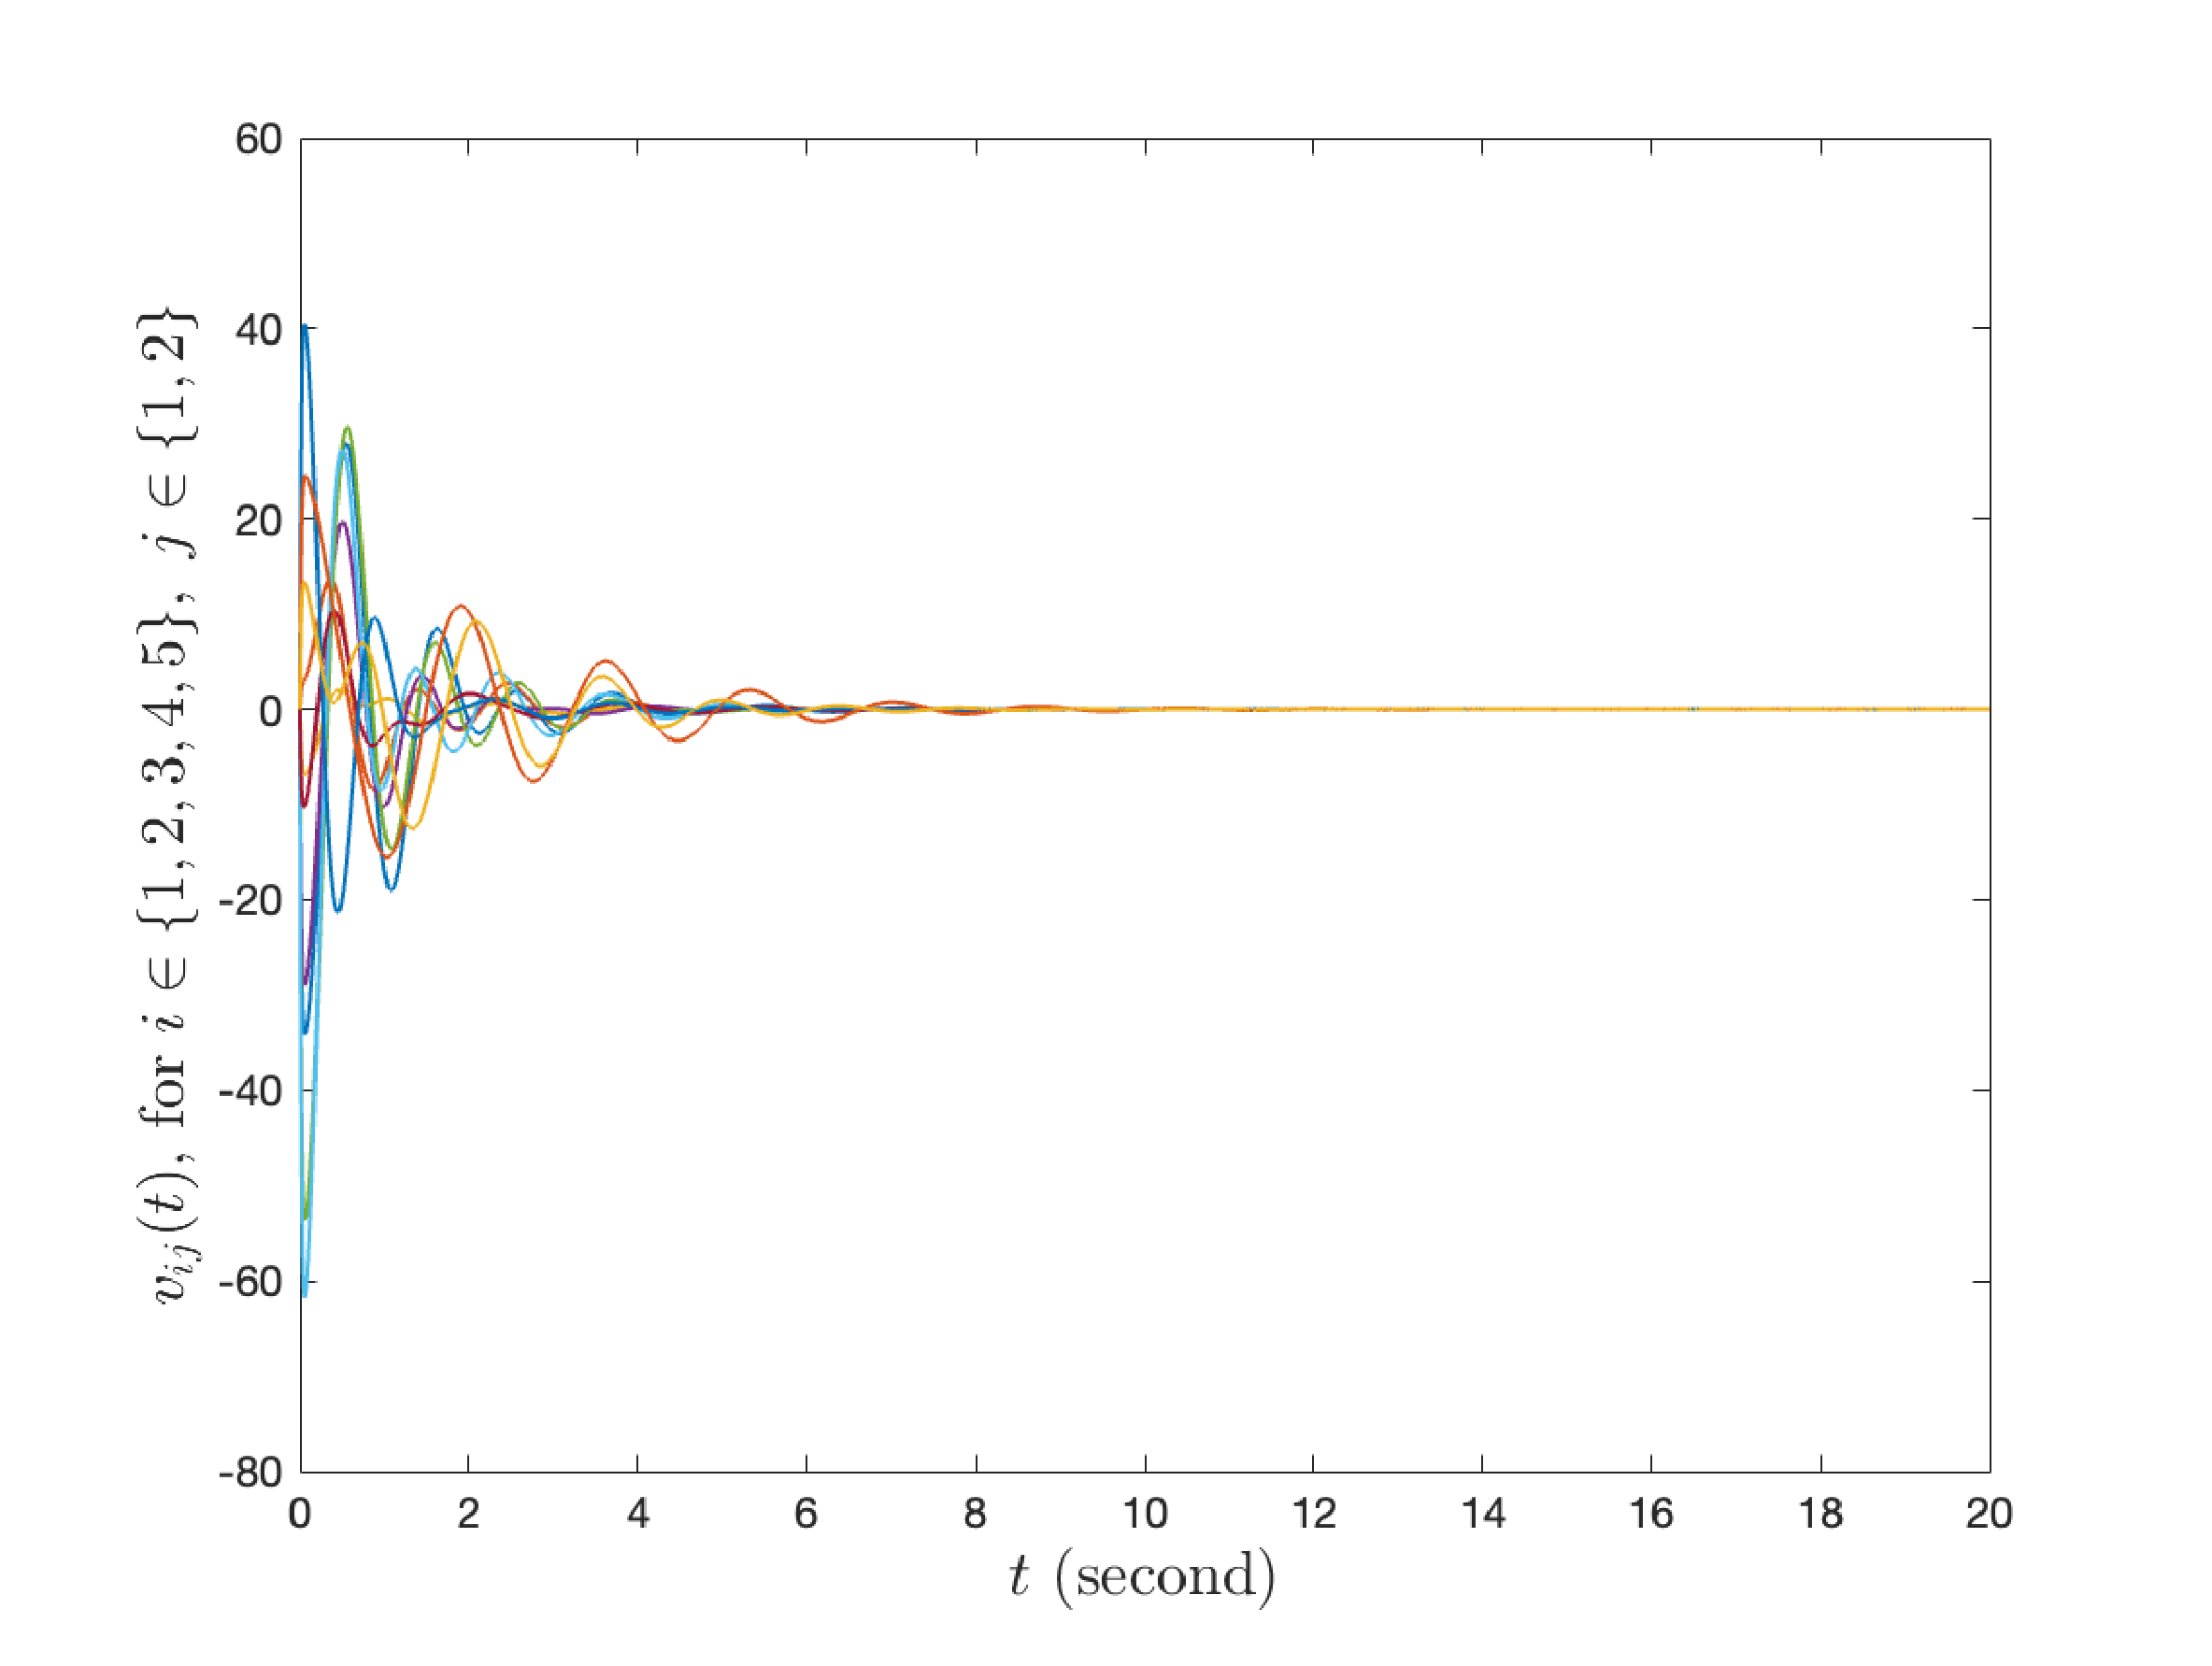
\includegraphics[width=0.45\textwidth]{img/vij.eps}
    \caption{Players' velocity-like state $v_{ij}$ for $i\in \{1,2,3,4,5\},~j\in \{1,2\}$.}
\end{figure}

It is found from Fig. 2, Fig. 3 and Fig. 4 that the proposed algorithm can drive the actions of all players to a small neighborhood of a Nash equilibrium point by adjusting the control gains properly, thereby verifying the conclusion of Theorem 1.

\section{CONCLUSIONS}
Anti-disturbance Nash equilibrium seeking algorithms for games with second-order disturbed distributed systems have been developed based on a chattering free continuous function method. It is theoretically proven that the actions of players can be achieved exponential convergence by an appropriate adjustment of control gains. Compared the strategy based on signum function \cite{9696299}, the Nash equilibrium seeking strategy of this paper is able to prevent chattering in practical engineering applications. It's worth mentioning that the proposed method in this paper does not require distributed estimation of all players' actions and some specific objective functions determined by the players, while the method in \cite{8985536} requires.

% \bibliographystyle{ieeetr}
% \bibliography{ref.bib}

\begin{thebibliography}{10}

    \bibitem{pozo2011finding}
    D.~Pozo and J.~Contreras, ``Finding multiple nash equilibria in pool-based markets: A stochastic epec approach,'' {\em IEEE Transactions on Power Systems}, vol.~26, no.~3, pp.~1744--1752, 2011.

    \bibitem{ratliff2016characterization}
    L.~J. Ratliff, S.~A. Burden, and S.~S. Sastry, ``On the characterization of local nash equilibria in continuous games,'' {\em IEEE transactions on automatic control}, vol.~61, no.~8, pp.~2301--2307, 2016.

    \bibitem{lou2015nash}
    Y.~Lou, Y.~Hong, L.~Xie, G.~Shi, and K.~H. Johansson, ``Nash equilibrium computation in subnetwork zero-sum games with switching communications,'' {\em IEEE Transactions on Automatic Control}, vol.~61, no.~10, pp.~2920--2935, 2015.

    \bibitem{stankovic2011distributed}
    M.~S. Stankovic, K.~H. Johansson, and D.~M. Stipanovic, ``Distributed seeking of nash equilibria with applications to mobile sensor networks,'' {\em IEEE Transactions on Automatic Control}, vol.~57, no.~4, pp.~904--919, 2011.

    \bibitem{liu2011stochastic}
    S.-J. Liu and M.~Krsti{\'c}, ``Stochastic nash equilibrium seeking for games with general nonlinear payoffs,'' {\em SIAM Journal on Control and Optimization}, vol.~49, no.~4, pp.~1659--1679, 2011.

    \bibitem{durr2013lie}
    H.-B. D{\"u}rr, M.~S. Stankovi{\'c}, C.~Ebenbauer, and K.~H. Johansson, ``Lie bracket approximation of extremum seeking systems,'' {\em Automatica}, vol.~49, no.~6, pp.~1538--1552, 2013.

    \bibitem{ding2019distributed}
    L.~Ding, Q.-L. Han, B.~Ning, and D.~Yue, ``Distributed resilient finite-time secondary control for heterogeneous battery energy storage systems under denial-of-service attacks,'' {\em IEEE Transactions on Industrial Informatics}, vol.~16, no.~7, pp.~4909--4919, 2019.

    \bibitem{wu2021resilient}
    J.~Wu, Y.~Zhu, Y.~Zheng, and H.~Wang, ``Resilient bipartite consensus of second-order multiagent systems with event-triggered communication,'' {\em IEEE Systems Journal}, 2021.

    \bibitem{ge2021dynamic}
    X.~Ge, S.~Xiao, Q.-L. Han, X.-M. Zhang, and D.~Ding, ``Dynamic event-triggered scheduling and platooning control co-design for automated vehicles over vehicular ad-hoc networks,'' {\em IEEE/CAA Journal of Automatica Sinica}, vol.~9, no.~1, pp.~31--46, 2021.

    \bibitem{ye2022distributed}
    M.~Ye, Q.-L. Han, L.~Ding, S.~Xu, and G.~Jia, ``Distributed nash equilibrium seeking strategies under quantized communication,'' {\em IEEE/CAA Journal of Automatica Sinica}, 2022.

    \bibitem{7888532}
    M.~Ye and G.~Hu, ``Distributed nash equilibrium seeking by a consensus based approach,'' {\em IEEE Transactions on Automatic Control}, vol.~62, no.~9, pp.~4811--4818, 2017.

    \bibitem{8093754}
    M.~Ye and G.~Hu, ``Distributed nash equilibrium seeking in multiagent games under switching communication topologies,'' {\em IEEE Transactions on Cybernetics}, vol.~48, no.~11, pp.~3208--3217, 2018.

    \bibitem{ye2021adaptive}
    M.~Ye and G.~Hu, ``Adaptive approaches for fully distributed nash equilibrium seeking in networked games,'' {\em Automatica}, vol.~129, p.~109661, 2021.

    \bibitem{7265050}
    W.-H. Chen, J.~Yang, L.~Guo, and S.~Li, ``Disturbance-observer-based control and related methods—an overview,'' {\em IEEE Transactions on Industrial Electronics}, vol.~63, no.~2, pp.~1083--1095, 2016.

    \bibitem{xie2000much}
    L.-L. Xie and L.~Guo, ``How much uncertainty can be dealt with by feedback?,'' {\em IEEE Transactions on Automatic Control}, vol.~45, no.~12, pp.~2203--2217, 2000.

    \bibitem{li2014disturbance}
    S.~Li, J.~Yang, W.-H. Chen, and X.~Chen, {\em Disturbance observer-based control: methods and applications}.
    \newblock CRC press, 2014.

    \bibitem{prabhakar2018trajectory}
    N.~Prabhakar, A.~Painter, R.~Prazenica, and M.~Balas, ``Trajectory-driven adaptive control of autonomous unmanned aerial vehicles with disturbance accommodation,'' {\em Journal of Guidance, Control, and Dynamics}, vol.~41, no.~9, pp.~1976--1989, 2018.

    \bibitem{namik2009disturbance}
    H.~Namik and K.~Stol, ``Disturbance accommodating control of floating offshore wind turbines,'' in {\em 47th AIAA aerospace sciences meeting including the new horizons forum and aerospace exposition}, p.~483, 2009.

    \bibitem{paradkar2004integration}
    A.~Paradkar, A.~Davari, A.~Feliachi, and T.~Biswas, ``Integration of a fuel cell into the power system using an optimal controller based on disturbance accommodation control theory,'' {\em Journal of Power Sources}, vol.~128, no.~2, pp.~218--230, 2004.

    \bibitem{9745491}
    X.-G. Guo, D.-Y. Zhang, J.-L. Wang, J.~H. Park, and L.~Guo, ``Observer-based event-triggered composite anti-disturbance control for multi-agent systems under multiple disturbances and stochastic fdias,'' {\em IEEE Transactions on Automation Science and Engineering}, vol.~20, no.~1, pp.~528--540, 2023.

    \bibitem{9547799}
    Y.~Wu and L.~Liu, ``Distributed average tracking for linear heterogeneous multi-agent systems with external disturbances,'' {\em IEEE Transactions on Network Science and Engineering}, vol.~8, no.~4, pp.~3491--3500, 2021.

    \bibitem{LU2020338}
    H.~Lü, W.~He, Q.-L. Han, X.~Ge, and C.~Peng, ``Finite-time containment control for nonlinear multi-agent systems with external disturbances,'' {\em Information Sciences}, vol.~512, pp.~338--351, 2020.

    \bibitem{zhang2013distributed}
    Y.~Zhang, Y.~Yang, Y.~Zhao, and G.~Wen, ``Distributed finite-time tracking control for nonlinear multi-agent systems subject to external disturbances,'' {\em International Journal of Control}, vol.~86, no.~1, pp.~29--40, 2013.

    \bibitem{9696299}
    M.~Ye, D.~Li, Q.-L. Han, and L.~Ding, ``Distributed nash equilibrium seeking for general networked games with bounded disturbances,'' {\em IEEE/CAA Journal of Automatica Sinica}, vol.~10, no.~2, pp.~376--387, 2023.

    \bibitem{ye2020distributed}
    M.~Ye, ``Distributed robust seeking of nash equilibrium for networked games: An extended state observer-based approach,'' {\em IEEE Transactions on Cybernetics}, vol.~52, no.~3, pp.~1527--1538, 2020.

    \bibitem{li2021distributed}
    D.~Li and M.~Ye, ``Distributed robust nash equilibrium seeking by unknown dynamics estimator based approaches,'' in {\em 2021 4th IEEE International Conference on Industrial Cyber-Physical Systems (ICPS)}, pp.~840--845, IEEE, 2021.

    \bibitem{8985536}
    B.~Huang, Y.~Zou, and Z.~Meng, ``Distributed-observer-based nash equilibrium seeking algorithm for quadratic games with nonlinear dynamics,'' {\em IEEE Transactions on Systems, Man, and Cybernetics: Systems}, vol.~51, no.~11, pp.~7260--7268, 2021.

    \bibitem{lewis2013cooperative}
    F.~L. Lewis, H.~Zhang, K.~Hengster-Movric, and A.~Das, {\em Cooperative control of multi-agent systems: optimal and adaptive design approaches}.
    \newblock Springer Science \& Business Media, 2013.

    \bibitem{10192924}
    P.~Wang, H.~Tian, D.~Huang, and T.~Huang, ``A continuous neural network adaptive controller for consensus of uncertain multi-agent systems,'' {\em IEEE Transactions on Emerging Topics in Computational Intelligence}, pp.~1--10, 2023.

\end{thebibliography}


\end{document}


